
%%%%%%%%%%%%%%%%%%%%%%%%%%%%%%%%%%%%%%%%%%%%%%%%%%%%%%%%%%
\chapter{Introduction}
\label{chapter_introduction}
%%%%%%%%%%%%%%%%%%%%%%%%%%%%%%%%%%%%%%%%%%%%%%%%%%%%%%%%%%

\begin{figure}
\centering

\includegraphics[width=1.0\textwidth]{figures/intro/unilever_w_neg_space.pdf} 
\caption[Unilever logo packing and its negative space]
{\label{fig_logo_packing} 
(a) The Unilever logo packing consists of 25 elements arranged inside an \newtext{estimated U-shaped container}. 
(b) \newtext{The red region, consisting of the remaining area not claimed by the elements, is referred to as negative space.}
}
\end{figure}

\begin{figure}
\centering
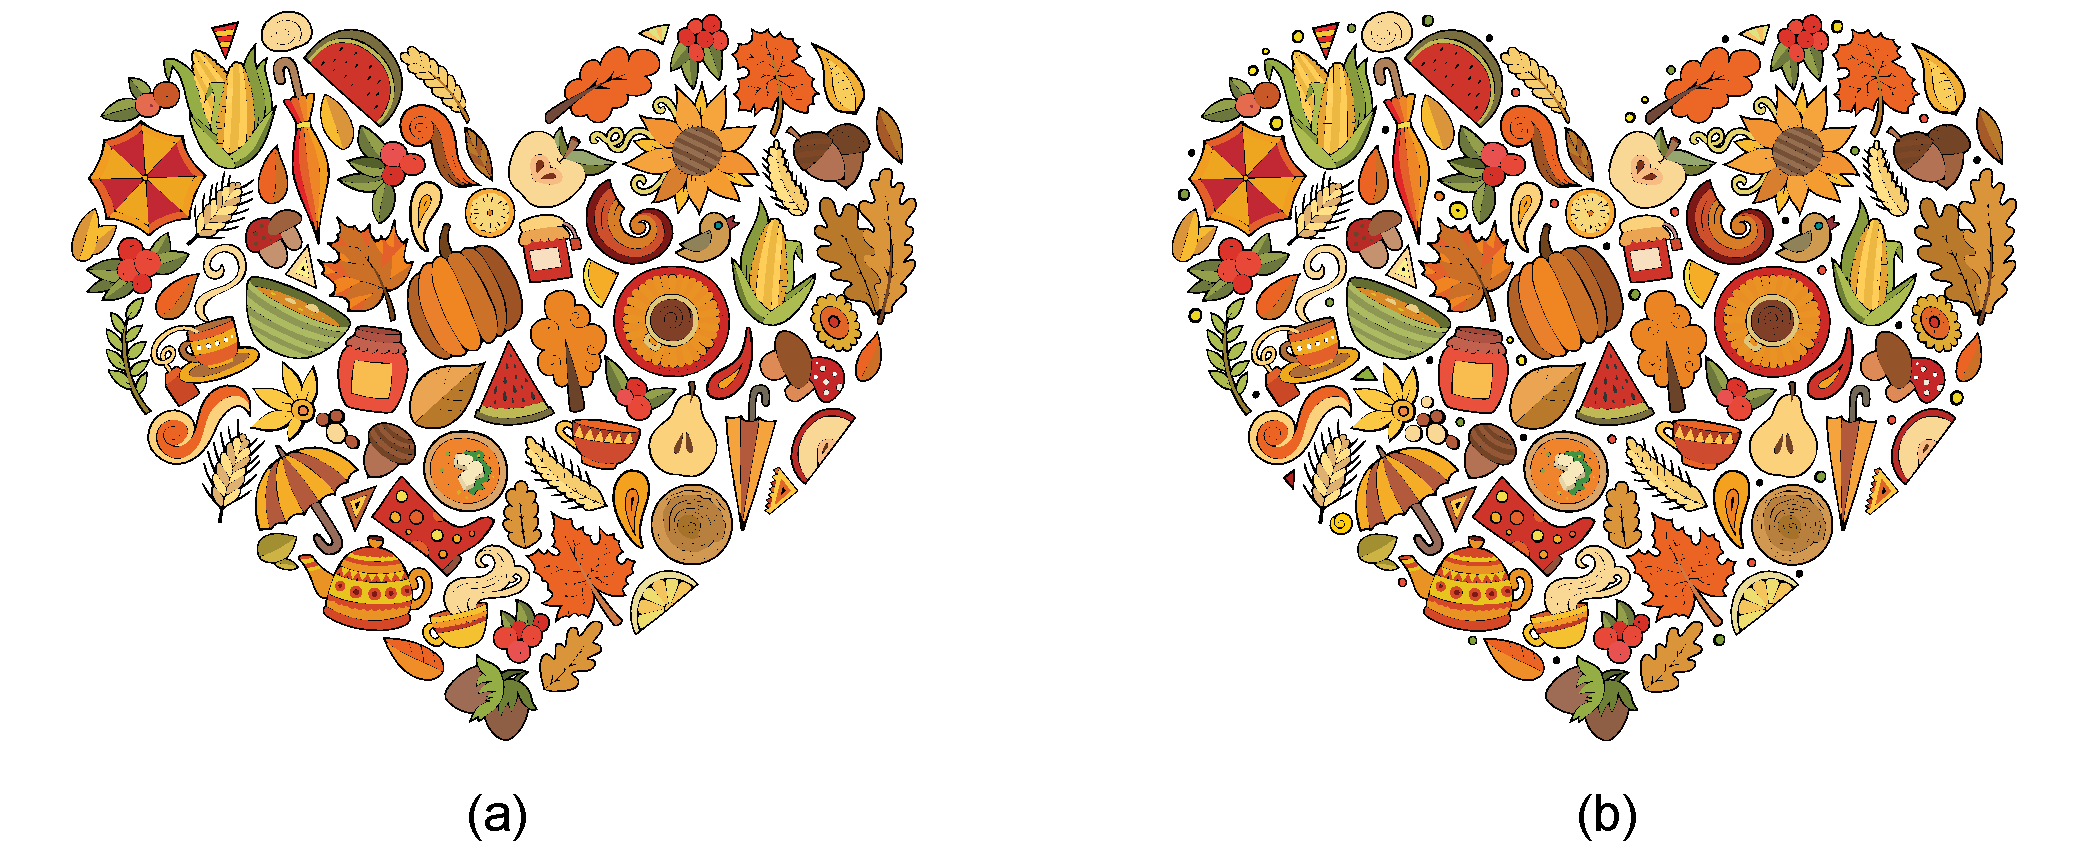
\includegraphics[width=1.0\textwidth]{figures/intro/primary_secondary.pdf}
\caption[Primary and secondary elements]{
  \label{fig_primary_secondary}
  \newtext
  {
  An autumn-themed packing created by Balabolka \nnewtext{on Shutterstock}. }
  (a) The packing with primary elements only.
  (b) Secondary elements are added. 
}
\end{figure}

\begin{figure}
\centering
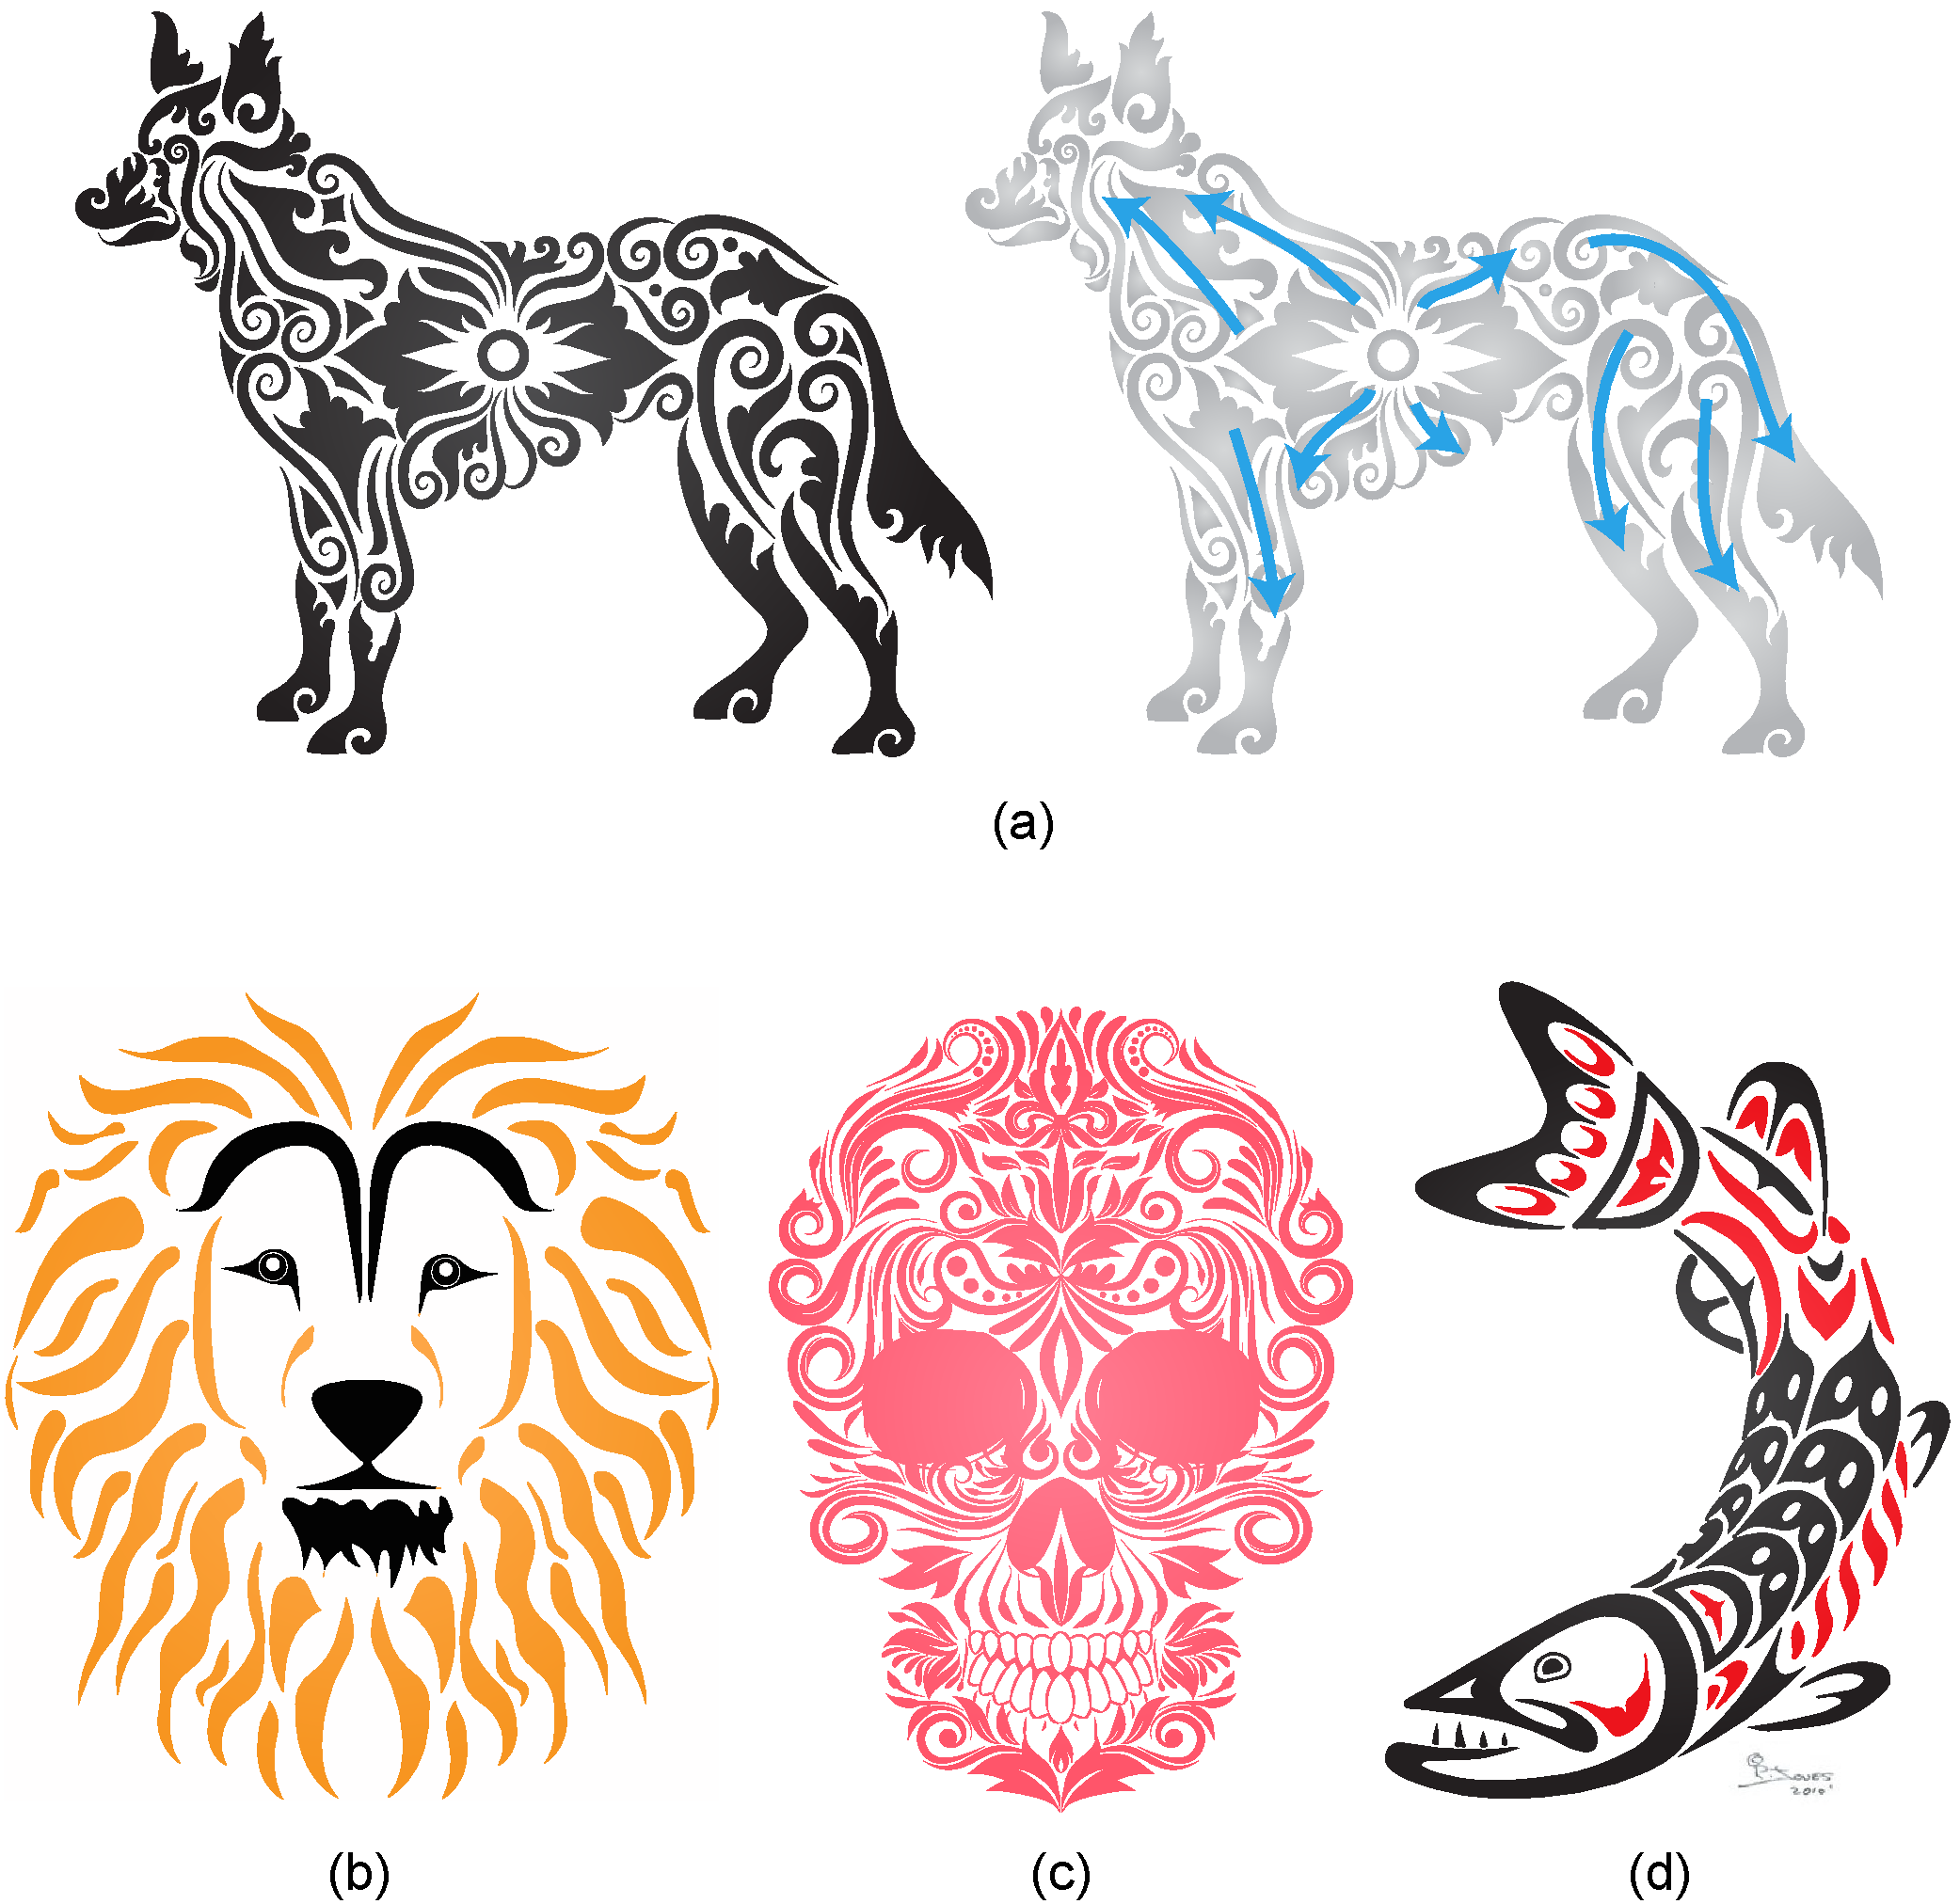
\includegraphics[width=1.0\textwidth]{figures/intro/dog_ornament_flow.pdf} 
\caption[Packings with flow visual styles]
{\label{fig_dog_flow} 
\newtext
{
Packings with \nnewtext{flow-based} visual styles:}
(a) Dog (by ComicVector703 on Shutterstock), 
including a visualization showing the flow directions of elements; 
(b) Lion (from StockUnlimited);  
(c) Skull (by alitdesign on Shutterstock).
(d) Fish in the style of Haida art (by Russ Jones, used with permission); 
 }
\end{figure}


%\begin{figure}
%\centering
%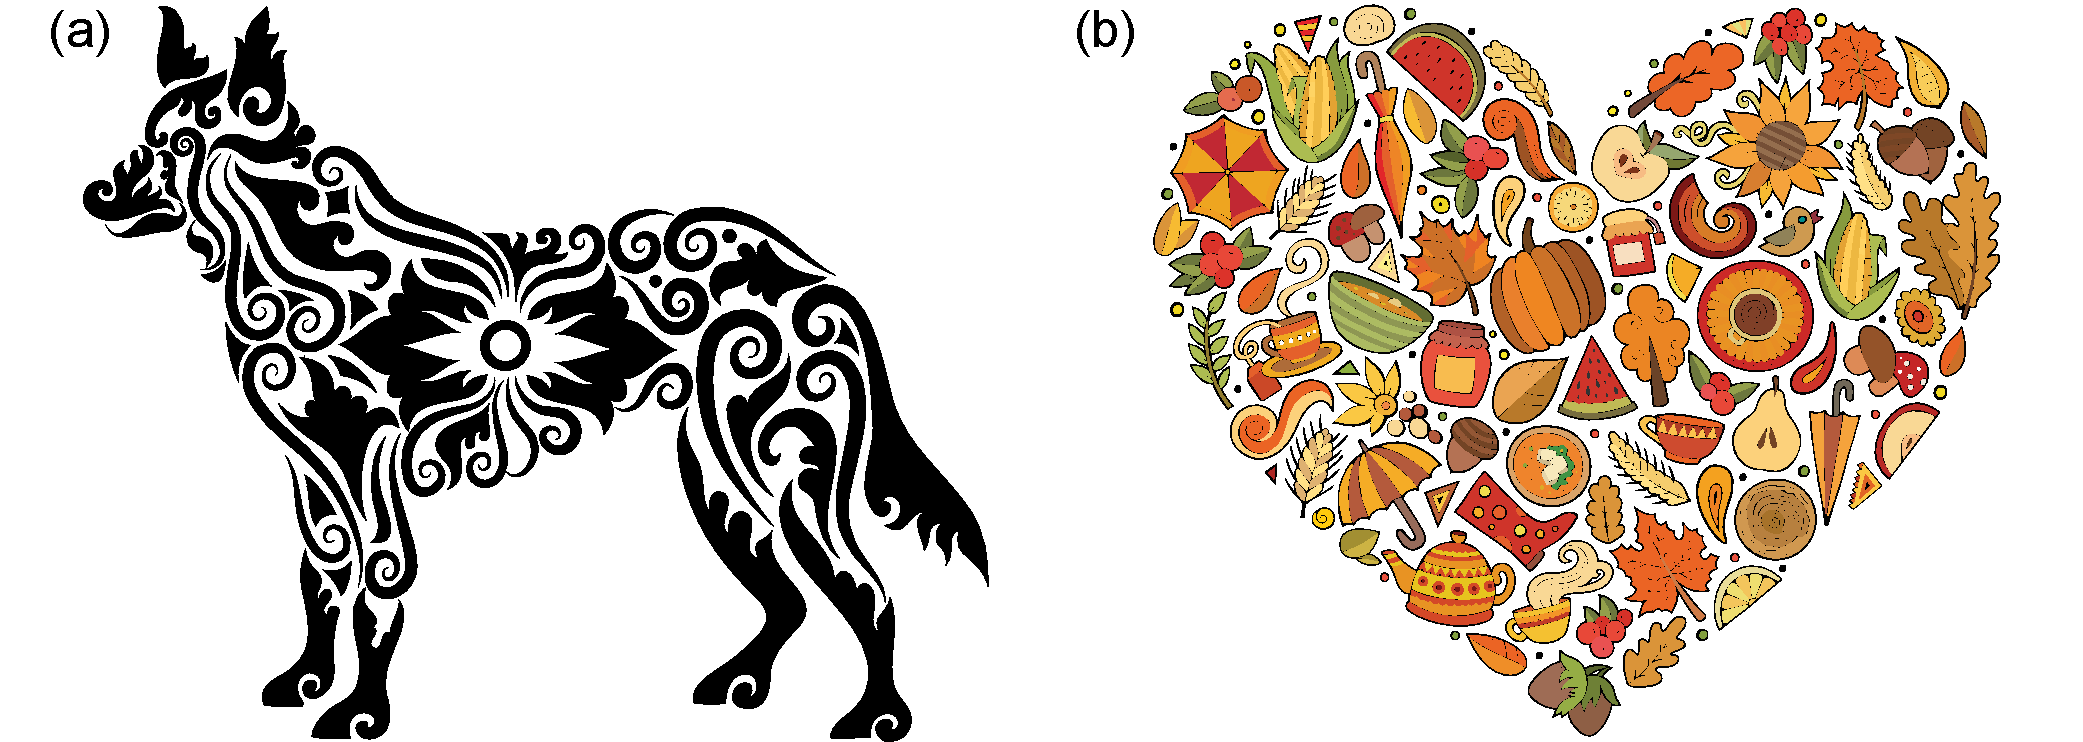
\includegraphics[width=1.0\textwidth]{figures/intro/balabolka_dog_flow.pdf} 
%\caption[Packings in graphic design]
%{\label{fig_graphic_designs} 
%\newtext
%{
%Two packing examples in graphic design.
%(a) A packing of autumn-themed elements, created by Balabolka.
%(b) A packing of abstract-shaped elements that create a flow visual style, created by ComicVector703.
%}
% }
%\end{figure}

\begin{figure}
\centering
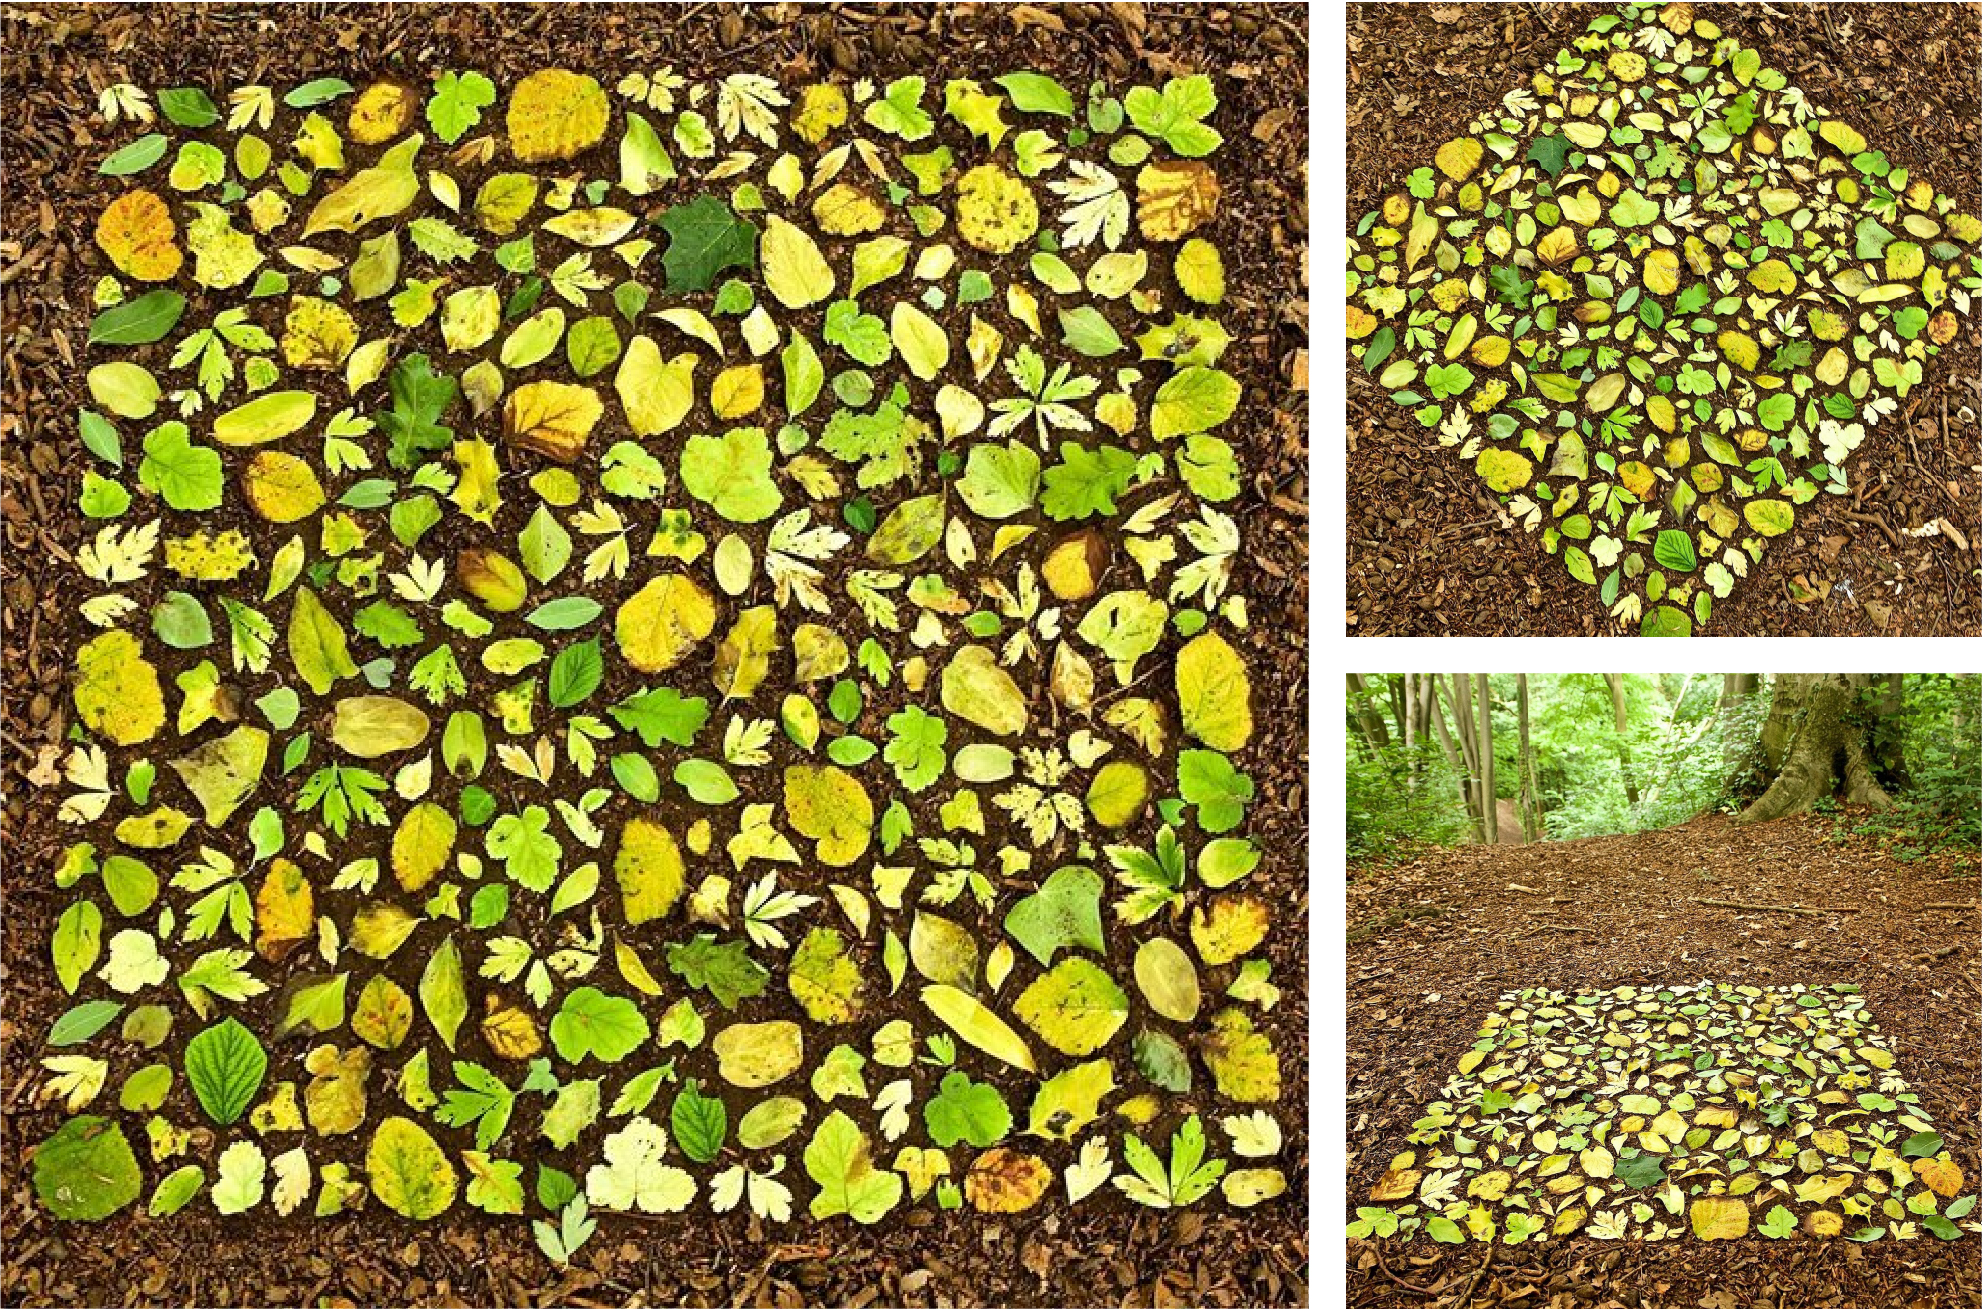
\includegraphics[width=1.0\textwidth]{figures/intro/woodland.jpg} 
\caption[A land art packing]
{\label{fig_woodland} 
\newtext
{
%A packing of leaves by James Brunt. 
A land art packing that is composed of leaves, created by James Brunt. 
Each leaf is oriented toward the center of the circle.
}
 }
\end{figure}

%\begin{figure}
%\centering
%\includegraphics[width=0.5\textwidth]{figures/intro/valve_lobby.jpg} 
%\caption{\label{fig_valve_lobby} 
%A packing installation in a lobby of a video game company. }
%\end{figure}

%\begin{figure}
%\centering
%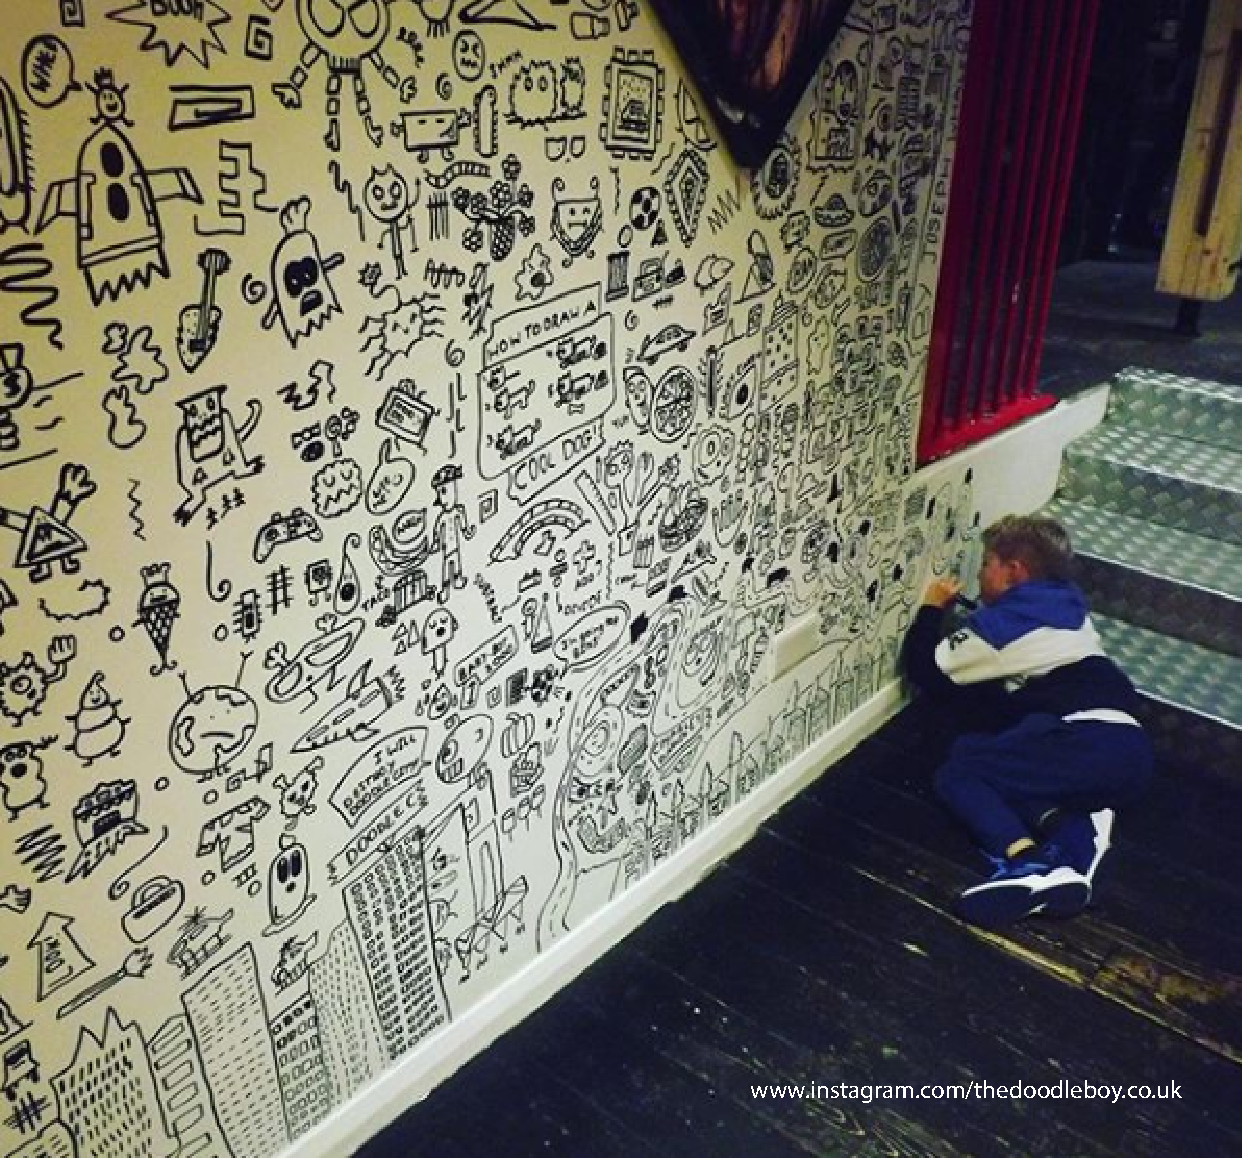
\includegraphics[width=0.5\textwidth]{figures/intro/doodle_boy.pdf} 
%\caption{\label{fig_doodle_boy} 
%Doodle boy. }
%\end{figure}

%\mynote{
%Thesis Statement (one or two sentences)
%\begin{packeditems}
%\item What is your thesis about and what have you done?
%\item If you have a hypothesis what is it?
%\item How will you test (prove/disprove) your hypothesis?
%\end{packeditems}
%}

%\mynote{align with boundary}

\newtext
{
A \textit{packing} is an arrangement of geometric
\textit{elements} within a \textit{container} region in the plane.
As an artistic composition, 
a packing can communicate a relationship between a whole and the parts that make it up.
Elements work together to communicate the overall container shape,
but each is large enough to be appreciated individually.
Elements are shapes like animals, plants, abstract geometry, or man-made objects.
Packings are popular in logo design, graphic design, and art.
Figure~\ref{fig_logo_packing}a shows the Unilever logo,
which is a 2D packing of elements arranged inside a U-shaped container.}


\newtext{The subset of the container that does not belong to any element is
called \textit{negative space} (Figure~\ref{fig_logo_packing}b).
We can also interpret negative space as separation and gaps between elements.
On the other hand, elements can be interpreted as \textit{positive space}.
In this thesis, we narrow our focus \nnewtext{to} packings without element overlaps,
which makes it easier to discuss positive and negative space without 
double counting the positive space.}

\newtext{The evenness of negative space plays an important role in packings.
Initially, an artist should arrange elements in \nnewtext{such} way that their boundaries interlock with each other,
causing the separation between neighboring elements to become roughly the same everywhere.
We refer \nnewtext{to elements} in the resulting packing as \textit{primary elements}.
However, the interlocking of primary elements is imperfect, and \nnewtext{artists will frequently place} smaller \textit{secondary elements} 
such as triangles or circles to reduce remaining large gaps,
\nnewtext{as shown in} the autumn-themed packing in Figure~\ref{fig_primary_secondary}.}

 
%\newtext{Elements can also be oriented to follow certain directions for aesthetic reasons.
%Figure~\ref{fig_graphic_designs}b is an ornamental packing
%of long thin elements that are bent and oriented outward from the center of the torso to create a flow visual style.
%Another example is shown in Figure \ref{fig_woodland}, which is a packing of leaves, each is oriented toward the center of the container.
%On both examples, the flow visual style gives an impression of progression and movements.}
\newtext{
\textbf{Design Principles:}
In studying packing designs, 
we have identified five high-level principles that are important
to the construction of packings:
}
\begin{items}%[leftmargin=*]
\item \textbf{Balance.} A composition does not exhibit too
  much variation in local amounts of positive and negative space.
  Typically, this goal is accomplished by limiting variation in 
  the diameters of elements (controlling the variation in
  positive space), and in ensuring that elements are spaced 
  evenly (controlling negative space).
  \nnewtext{The primary elements Figure~\ref{fig_primary_secondary} come in a range of sizes, but none so extreme that they stand out. 
  Additionally, interlocking elements lead to channels of negative space that are roughly constant in width.}

\item \textbf{Flow.} In local parts of a composition, the elements
  are oriented to communicate a sense of directionality or flow.
  \newtext{Examples in Figure~\ref{fig_dog_flow} exhibit 
  some amount of flow.  In the dog, many elements appear to flow
  outward from the flower in the center of the torso, and then
  up the neck and down into the legs.  The scales and other elements
  on the fish flow along the length of its body.  In the lion and skull,
  elements flow horizontally outward from a central axis of symmetry,
  suggesting fur in the case of the lion.  
  Another example is shown in Figure \ref{fig_woodland}, which is a packing of leaves
  that are oriented toward the center of the container.}   
  Flow  adds visual interest to a composition, engaging the viewer 
  by providing a sense of progression and movement through elements.

\item \textbf{Uniformity Amidst Variety.} Repeated elements must balance
  between two opposing forces.  \textit{Uniformity} 
  aims for an overall unity of design; \textit{variety}
  seeks to break up the monotony of
  pure repetition.  Elements should be permitted to vary in shape,
  but in a controlled way.  We refer to this principle
  as \textit{uniformity amidst variety}, a term borrowed from 
  philosopher Francis Hutcheson~\cite{Hutcheson1729}.
  Gombrich also writes eloquently on the role of variation in 
  design~\cite{Gombrich}.
  \newtext{
  The Unilever packing in Figure~\ref{fig_logo_packing} has the elements drawn with a similar curvy design. 
  In Figure~\ref{fig_primary_secondary}, the elements are autumn-themed shapes and are convex or near convex. 
  In Figure~\ref{fig_dog_flow}, the dog's spirals and the
  fish's scales both obey this principle.  The lion and skull do as well,
  except that half of the elements are reflected copies of the other
  half, across a vertical line through the center of the composition.
  This repetition emphasizes the bilateral symmetry in the design.
  The land art packing in Figure~\ref{fig_woodland} \nnewtext{has} the most uniformity \nnewtext{of these} examples:
  the leaves have \nnewtext{similar shapes} and the composition conveys the radial symmetry.
  The artist added some amount of variety by using different leaf sizes and colors.
  }

\item \textbf{Fixed Elements.} Compositions use a small number of fixed
  elements to solve specific design problems or provide focal points.
  In any figurative drawing, eyes serve as a powerful focal point;
  every example in Figure~\ref{fig_dog_flow} has eyes drawn
  in as unique elements
  (the dog's eye is expressed via a carefully placed spiral).  Other
  situations that call for specialized shapes include the dog's paws,
  the fish's teeth and fins, 
  the lion's eyes and nose, %%% REZA BACKUP
  and the skull's teeth.
  Sharp variation in the balance of positive and negative space
  can also be used to emphasize a focal point,
  as in the fish's head and the lion's face that contain considerable amount of empty space.

\item \textbf{Boundaries.} In many ornamental packings, elements are
  carefully arranged to conform to and emphasize container boundaries.
  \nnewtext{Elements in the Unilever packing (Figure~\ref{fig_logo_packing}) and the autumn-themed packing (Figure~\ref{fig_primary_secondary})
  demonstrate this principle most clearly: }we can easily
  fill in the gaps between elements to form a mental image of a continuous
  outline.
  In Figure~\ref{fig_dog_flow}a, the dog's elements are also well aligned to indicate the
  container shape. 
  However, this rule is not universal.  
  The lion packing in Figure~\ref{fig_dog_flow}b artfully subverts it with elements that flow outward to an
  indistinct boundary, helping to convey the appearance of fur.
  %The fish demonstrates this principle most clearly: we can easily
  %fill in the gaps between elements to form a mental image of a continuous
  %outline.  The dog's elements are also well aligned to indicate the
  %container shape.  
\end{items}


\newtext{There has been a moderate amount of past research in computer
graphics, particularly in the field of non-photorealistic rendering,
on the generation of packings, or mosaics.  
See Chapter~\ref{chapter_related_work} for specific examples.  
However,  most techniques pack elements via rigid transformations, leading to
uneven element distribution and overlaps.  
}

\newtext{
Jigsaw Image Mosaics~\cite{Kim2002} and collages based on the Pyramid of Arclength
Descriptor~\cite{Kwan2016} are \textit{data-driven}.
These techniques rely on a large library of elements, so that given an
area to fill in a partial composition, there is likely to be an
element in the library with a compatible shape.  The challenge is 
\textit{finding} compatible elements,
which requires designing a shape matching technique that is fast and robust.
Additionally, they cannot guarantee to find a compatible element
at every iteration, and elements typically do not fit perfectly with each other 
or the container boundary.
The remedy here is providing more data with increased computation time.
However, a large library may not be feasible or artistically desirable.
If an artist wants a packing of hand-drawn cats, and a data-driven approach 
cannot find a good result with ten cat shapes, 
the artist may not want to draw 100 or 1000 cats to ensure a better fit.
}

\newtext{In this thesis, we propose \textit{deformation-driven} methods.
Instead of finding compatible elements,
we \textit{create} compatible elements through deformation; 
these deformed elements can adapt to the shapes of neighboring elements and the container boundary.
We allow elements to deform in a controlled way,
to trade off between the evenness of the element distribution and 
the deformations of the individual elements.
By building an algorithm with a controllable deformation model at its core, we achieve a
more even distribution of negative space, 
and we require only a small library of element shapes.}
\newtext{
Deformation-driven methods also allow us to work toward the principle of uniformity amidst variety.
We can achieve a degree of uniformity by using repeated copies of a small library of elements, but balance that uniformity with
variety by deforming those elements. 
We believe that there is a value in deformation that can generate plausible families of related elements from a single input shape.
}

%\newtext
%{
%Deformation-driven methods also allow us to work toward a design principle called \textit{uniformity amidst variety}~\cite{Hutcheson1729, Gombrich}. 
%\textit{Uniformity} aims for an overall unity of design and 
%\textit{variety} seeks to break up the monotony of pure repetition.
%We can achieve a degree of uniformity by using repeated copies of a small library of elements, but balance that uniformity with
%variety by deforming those elements. 
%We believe that there is a value in deformation that can generate plausible families of related elements from a single input shape.
%}

\newtext{
In this thesis, many of our techniques are inspired by physical simulations.
We create an element representation 
that can be deformed by pseudo-physical forces. 
\nnewtext{Our goal is not to contribute to research on physics-based animation, but to use a} physical simulation as an optimization process that allows us to
reach a physical equilibrium where the resulting packing has approximately uniform
distribution of both positive and negative space.
}

\newtext
{
% https://learningenglish.voanews.com/a/the-more-i-practice-the-more-i-remember/4995040.html
The perceived packing quality is closely tied to the evenness of negative space.
The more the elements interlock, the more even the negative space. 
We are interested in quantitative measurements of evenness 
in order to evaluate and compare packing algorithms.
In this thesis we discuss several possible measurements of 
evenness based on methods from spatial statistics.
}

\textbf{Contributions:} \newtext
{
In this thesis, we develop three specific deformation-driven packing methods, 
and then study investigate the quantitative evaluation of packing quality in greater detail:
\begin{enumerate}
\item FLOWPAK is a packing method that deforms long thin elements to follow a user-defined vector field (Chapter~\ref{chapter_flowpak}).
\item RepulsionPak is a packing method that utilizes repulsion forces to distribute and deform elements,
	each is represented as a mass-spring system (Chapter~\ref{chapter_repulsionpak}).
\item AnimationPak is a method to pack 2D animated elements inside a static 2D container. 
	Each element is an extruded 3D shape in a spacetime domain 
	and we view the animated packing problem as a 3D packing in that domain.
	(Chapter~\ref{chapter_animationpak}). 
\item  Quantitative metrics for measuring the evenness of negative space: spherical contact probabilities,
histograms of the distance transforms, and the overlap functions (Chapter~\ref{chapter_qualitative_metrics}). 
\end{enumerate}
}

%\begin{labeling}{alligator}
%\item [ant] really busy all the time
%\item [chimp] likes bananas
%\item [alligator] very dangerous animal, sharp teeth, long
%muscular tail and a bit of text that is longer than one
%line and shows the alignment of text quite nicely
%\end{labeling}


%\mynote{TODO: Copy from comp\_2}
%A \textit{packing} is an arrangement of 2D geometric
%\textit{elements} within a \textit{container} region in the plane.
%Packings are popular in art, ornamentation, and graphics design.
%Figure ~\ref{fig_logo_packings}\ref{fig_graphics_designs}\ref{fig_woodland}\ref{fig_valve_lobby}\ref{fig_doodle_boy} show several packing examples.
%They can effectively convey a relationship between a unified whole (the
%container shape) and its many sub-parts (the elements).

%\mynote{maybe put negative space to the background section}
%Elements are shapes like animals,
%plants, geometric forms, or man-made objects.
%An artist distributes elements so that they communicate
%the shape of the container. 
%The subset of the container that does not belong to any element is
%called \textit{negative space}
%(Fig.~\ref{packing_example}, right).
%We can also interpret negative space as separation and gaps between elements.
%The evenness of negative space plays an important role in 
%packings.  
%The artist should arrange elements in a way that their boundaries interlock with each other,
%causing the separation between neighbouring elements to become roughly the same everywhere.
%As the elements in a packing become perfectly interlocked,
%the packing turns into a \textit{tiling}: a set of elements that exactly
%fill a container with no overlaps and no negative space (Fig.~\ref{related_work_images}b).



%\mynote{Motivation, Why is this problem you've worked on important}
%\mynote{Goals / Objectives, What are you trying to do and why? 
%How will you or the reader know if or when you've met your objectives?}


%\mynote{
%Contributions, What is new, different, better, significant? Why is the world a better place because of what you've done? What have you contributed to the field of research?  What is now known/possible/better because of your thesis?
%}



%\mynote {Explain briefly FLOWPAK, RepulsionPak, and AnimationPak.}